\documentclass[exb]{exercise_5.0}

\deadline{16.12.2024}

\begin{document}

\section{Local gauge invariance of the Schrödinger equation}
Applying the transformation to the right hand side yields:
\begin{align*}
    i D_0' \Psi' &= i \hug{\pp{}t + iQV'} e^{iQ\alpha(t,x)}\Psi\\
    &= i \hug{\pp{}t + iQ\hug{V-\p_t \alpha}} e^{iQ\alpha(t,x)}\Psi\\
    &= i \hug{\psi \p_t +  \p_t \psi + iQ\hug{V-\p_t \alpha}\psi }e^{iQ\alpha(t,x)} \\
    &= i \hug{iQ(\p_t\alpha) \psi +  \p_t \psi + iQ\hug{V-\p_t \alpha}\psi }e^{iQ\alpha(t,x)} \\
    &= e^{iQ\alpha(t,x)} i \hug{\p_t + iQV  }\psi \\
    \Aboxed{i D_0' \Psi'  &= e^{iQ\alpha(t,x)} i D_0\psi}
\end{align*}
And to the left hand side:
\begin{align*}
    D_x' \psi' &= \hug{-\pp{}x + iQA'}\psi'\\
    &= \hug{-\pp{}x + iQ\hug{A+ \p_x \alpha}} e^{iQ\alpha(t,x)} \psi\\
    &= \hug{-\p_x \psi - \psi \p_x + iQ\hug{A+ \p_x \alpha}\psi} e^{iQ\alpha(t,x)} \\
    &= \hug{-\p_x \psi - iQ (\p_x\alpha )\psi  + iQ\hug{A+ \p_x \alpha}\psi} e^{iQ\alpha(t,x)} \\
    &= e^{iQ\alpha(t,x)} \hug{-\p_x + iQA} \psi\\
    &= e^{iQ\alpha(t,x)} D_x \psi\\
    \\
    \Aboxed{D_x'^2\psi'
    &= D_x'\hug{ e^{iQ\alpha(t,x)} D_x \psi} = e^{iQ\alpha(t,x)} D_x^2 \psi}
\end{align*}
All in all this implies that the Schrödinger equation is locally gauge invariant:
\begin{align*}
    \frac1{2m} (i D_x')^2 \psi' &= i D_0' \Psi'\\ 
    e^{iQ\alpha(t,x)} \frac1{2m} (i D_x)^2 \psi &= e^{iQ\alpha(t,x)} i D_0' \Psi'\\ 
    \hug{e^{iQ\alpha(t,x)} \neq 0}\quad \frac1{2m} (i D_x)^2 \psi &= i D_0 \Psi\\ 
\end{align*}

\section{Gauge invariance and photon mass}
\subsection{}
\begin{align*}
    j^\mu &= \p_\nu \p^\nu \Lambda'^\mu - \p^\mu \p^\nu \Lambda'_\nu\\
     &= \p_\nu \p^\nu (\Lambda^\mu - \p^\mu\alpha) - \p^\mu \p^\nu (\Lambda_\nu - \p_\nu\alpha)\\
     &= \p_\nu \p^\nu \Lambda^\mu - \p^\mu \p^\nu \Lambda_\nu - \p_\nu \p^\nu  \p^\mu\alpha + \p^\mu \p^\nu \p_\nu\alpha\\
     &= \p_\nu \p^\nu \Lambda^\mu - \p^\mu \p^\nu \Lambda_\nu - \p^\mu \p_\nu \p^\nu \alpha + \p^\mu \p_\nu \p^\nu\alpha\\
     &= \p_\nu \p^\nu \Lambda^\mu - \p^\mu \p^\nu \Lambda_\nu
\end{align*}
i.e the wave equation is invariant under the gauge transformation $A^\mu \to A^\mu - \p^\mu \alpha$. 

\subsection{}
\begin{align*}
    j^\mu &= (\p_\nu \p^\nu + m^2) \Lambda'^\mu - \p^\mu \p^\nu \Lambda'_\nu\\
    &= \p_\nu \p^\nu \Lambda'^\mu- \p^\mu \p^\nu \Lambda'_\nu  + m^2 \Lambda'^\mu\\
    &= \p_\nu \p^\nu \Lambda^\mu- \p^\mu \p^\nu \Lambda_\nu  + m^2 \Lambda'^\mu\\
    0 &= m^2 \underbrace{\Lambda'^\mu}_{\not\equiv 0}
\end{align*}
i.e. wave equation for a massive vector field is only invariant under the same gauge transformation for $m=0$.

\section{Higgs factory}
\subsection{}
Electrons have no inner structure, which means that the initial state of a $e^+e^-$ collision is known, where as with a $p\bar p$ the quarks constituents have different energy levels resulting in a variety of possible inital states. Another advantage is that $e^+e^-$ colliders produce fewer hadronic backgrounds.

\subsection{}
The minimum center of mass energy has to suffice to produce a non virtual $Z$ and higgs boson:
\begin{align*}
    \sqrt{s\sub{min}} &= m_Z + m_H \approx 216\u{GeV}
\end{align*}

\subsection{}
The $e^+e^-$ collision produces a $Z$ which radiates a higgs boson. The Feynman-diagram of this production is:
\begin{figure}[H]
    \centering
    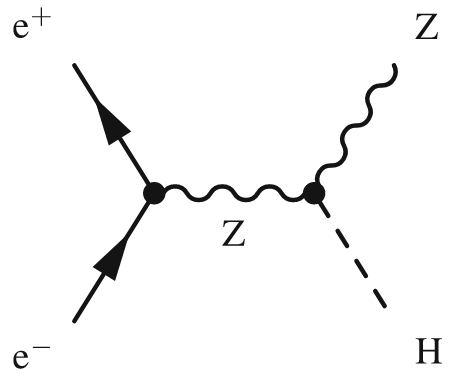
\includegraphics[width=.4\textwidth]{Higgsstrahlung.png}
\end{figure}

The heaviest fermion decay that can happen non virtually is $H \to b \bar b$, with the following feynman diagram:
\begin{figure}[H]
    \centering
    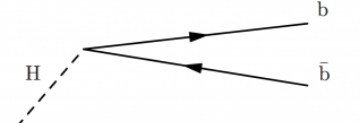
\includegraphics[width=.4\textwidth]{higgs2bottom.png}
\end{figure}

While the $Z$ decays either into two leptons $Z\to l\bar l$ or two quarks $Z\to q\bar q$:
\begin{figure}[H]
    \centering
    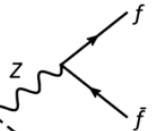
\includegraphics[width=.3\textwidth]{Z2fermion.png}
\end{figure}

The experimental signature is therefore:
\begin{enumerate}
    \item a pair of $b$-jets with invariant mass of $m_H$, correspoding to the Higgs 
    \item a pair of leptons or quark jets with invariant masses matching the $Z$-Bosons mass $m_Z$.
\end{enumerate}

\subsection{}
It follows from conservation of four-momentum that:
\begin{align*}
    p' &= p\\
    p_{e^+} + p_{e^-} &= p_Z + p_H\\
    \Aboxed{p_H &= p_{e^+} + p_{e^-} - p_Z}
\end{align*}
The mass is then given by:
\begin{align*}
    m_H^2 &= p_H^2\\
    &= (p_{e^+} + p_{e^-} - p_Z)^2\\
    &= (p_{e^+} + p_{e^-})^2 - 2(p_{e^+} + p_{e^-})p_Z + p_Z^2\\
    &= s - 2(p_{e^+} + p_{e^-})p_Z + m_Z^2\\
    \qte{(CoM frame)}&= s - 2(\sqrt s, \v 0)\cdot(E_Z, \v p_Z) + m_Z^2\\
    \Aboxed{m_H &= \sqrt{s - 2 E_Z \sqrt s + m_Z^2}}
\end{align*}
This relation can be used to calculate the Higgs mass without reconstructing the decay product of the Higgs boson. One just has to measure the center-of-mass energy $\sqrt m$ along with the energy of the $E_Z$ (assuming $m_Z$ is known with sufficient accuracy).

\section{Neutrino oscillations}
\subsection{}
\begin{align*}
    \binom{\ket{\nu_\mu}}{\ket{\nu_\tau}} &= \underbrace{\m{\cos\theta& \sin\theta\\-\sin\theta&\cos\theta}}_R \binom{\ket{\nu_2}}{\ket{\nu_3}}\\
    \\
    P_{\nu_\mu\to \nu_\mu} (t) 
    &= \abs{\braket{\nu_\mu}{\psi(t)}}^2\\
    &= \abs{\bra{\nu_\mu} e^{-iHt/\hbar}\ket{\nu_\mu}}^2\\
    \hug{E := \diag(E_2,E_3)}\quad &= \abs{\bra{\nu_\mu} R e^{-iEt/\hbar}R^\dagger \ket{\nu_\mu}}^2\\
    (\te{sympy})\quad&= \left(e^{\frac{i E_{2} t}{\hbar}} \cos^{2}{\left(\theta \right)} + e^{\frac{i E_{3} t}{\hbar}} \sin^{2}{\left(\theta \right)}\right) \left(e^{- \frac{i E_{3} t}{\hbar}} \sin^{2}{\left(\theta \right)} + e^{- \frac{i E_{2} t}{\hbar}} \cos^{2}{\left(\theta \right)}\right)\\
    &= \hug{\cos^2\theta+ \sin^2\theta e^{i(E_2 - E_3) t/\hbar}}\hug{\cos^2\theta+ \sin^2\theta e^{-i(E_2 - E_3) t/\hbar}}\\
    &= \cos^4\theta + \sin^4\theta + \sin^2\theta\cos^2\theta \hug{e^{i(E_2 - E_3) t/\hbar} + e^{-i(E_2 - E_3) t/\hbar}}\\
    &= \cos^4\theta + \sin^4\theta + 2\sin^2\theta\cos^2\theta \cos\hug{(E_2 - E_3) t/\hbar}\\
    &= \frac{\cos(4\theta) + 3}{4} + \frac{1-\cos(4\theta)}{4}\cos\hug{(E_2 - E_3) t/\hbar}\\
    &= \frac{\cos(4\theta) + 3}{4} + \frac{1-\cos(4\theta)}{4}\hug{1- 2\sin^2\hug{\frac {E_2 - E_3}2 t/\hbar}}\\
    &= 1 - \frac{1-\cos(4\theta)}{2}\sin^2\hug{\frac {E_2 - E_3}2 t/\hbar}\\
    &= 1 - \sin^2(2\theta)\sin^2\hug{\frac {E_2 - E_3}2 t/\hbar}
\end{align*}
  
\subsection{}
The code is appended on the last pages.
\begin{align*}
    P_{\nu_\mu\to \nu_\mu} (t) = 1 - \sin^2(2\theta)\sin^2\hug{\frac{\Delta m^2 L }{4 E}}
\end{align*}
The conversion factor from km to 1/eV can be derived as:
\begin{align*}
    \hbar c &= 197 \u{MeV} \cdot \u{fm} = 197\E{6} \u{eV} \E{-18}\u{km}\\
    \u {km} &= \frac{\hbar c}{197 \E{-12}} \ufrac1{eV} \approx 5.076\E{9} \ufrac1{eV}
\end{align*}
\begin{figure}[H]
    \centering
    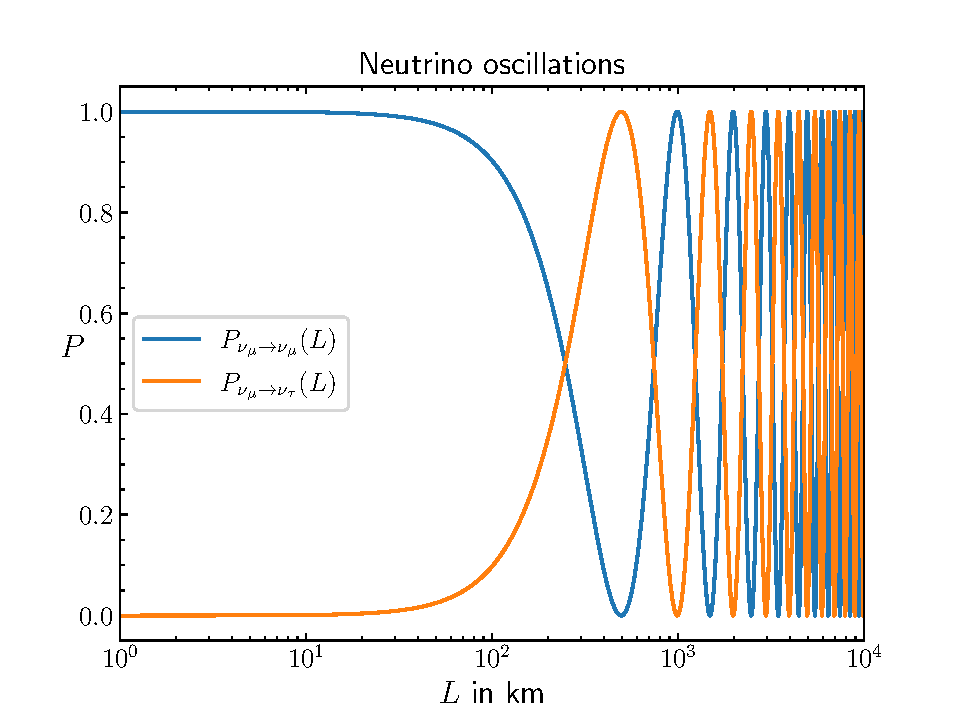
\includegraphics[width=.8\textwidth]{neutrino_oscillations.pdf}
    \caption{resulting plot}
\end{figure}

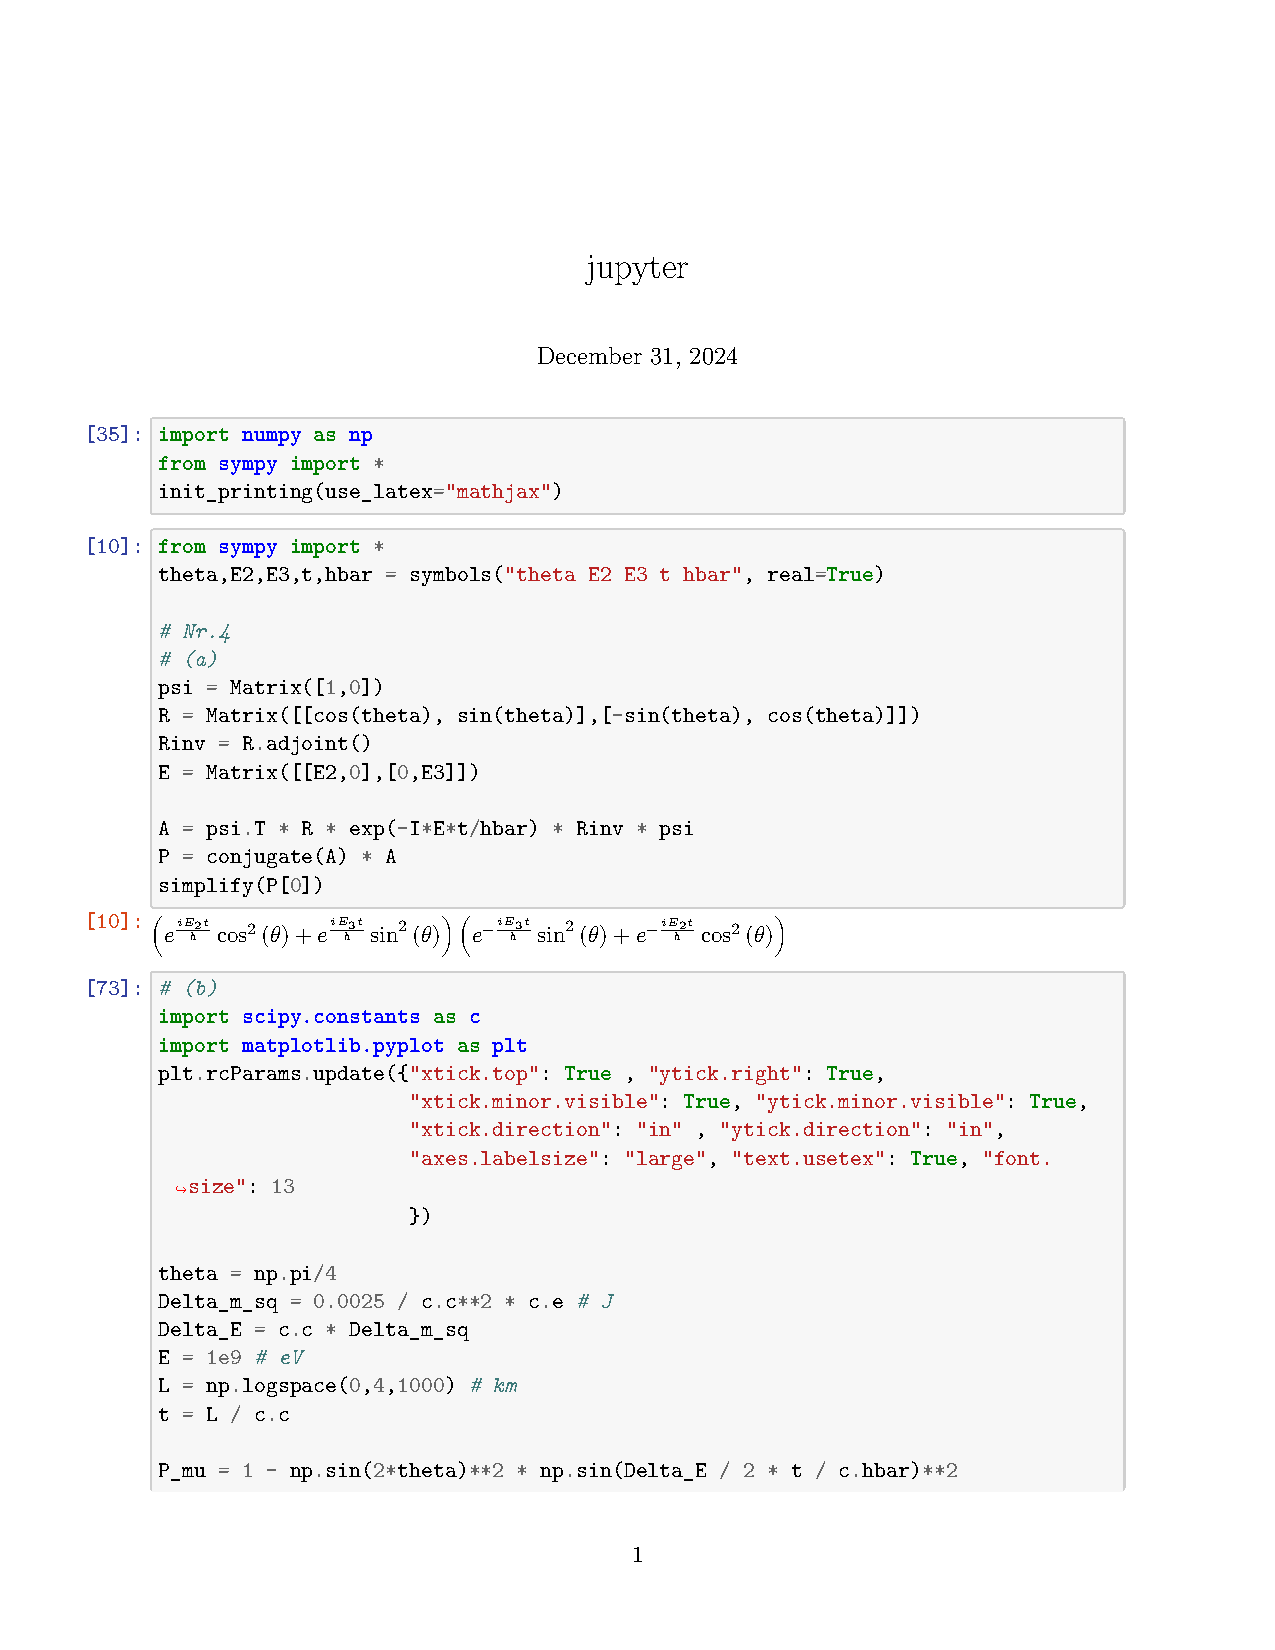
\includepdf[pages=-]{jupyter.pdf}

\end{document}